\documentclass[nooutcomes]{ximera}
%\documentclass[space,handout,nooutcomes]{ximera}

% For preamble materials

\usepackage{pgf,tikz}
\usepackage{mathrsfs}
\usetikzlibrary{arrows}
\usepackage{framed}
\usepackage{amsmath}
\pgfplotsset{compat=1.17}

\def\fixnote#1{\begin{framed}{\textcolor{red}{Fix note: #1}}\end{framed}}  % Allows insertion of red notes about needed edits
%\def\fixnote#1{}

\def\detail#1{{\textcolor{blue}{Detail: #1}}}   

\pdfOnly{\renewenvironment{image}[1][]{\begin{center}}{\end{center}}}

\graphicspath{
  {./}
  {chapter1/}
  {chapter2/}
  {chapter4/}
  {proofs/}
  {graphics/}
  {../graphics/}
}

\newenvironment{sectionOutcomes}{}{}


%%% This set of code is all of our user defined commands
\newcommand{\bysame}{\mbox{\rule{3em}{.4pt}}\,}
\newcommand{\N}{\mathbb N}
\newcommand{\C}{\mathbb C}
\newcommand{\W}{\mathbb W}
\newcommand{\Z}{\mathbb Z}
\newcommand{\Q}{\mathbb Q}
\newcommand{\R}{\mathbb R}
\newcommand{\A}{\mathbb A}
\newcommand{\D}{\mathcal D}
\newcommand{\F}{\mathcal F}
\newcommand{\ph}{\varphi}
\newcommand{\ep}{\varepsilon}
\newcommand{\aph}{\alpha}
\newcommand{\QM}{\begin{center}{\huge\textbf{?}}\end{center}}

\renewcommand{\le}{\leqslant}
\renewcommand{\ge}{\geqslant}
\renewcommand{\a}{\wedge}
\renewcommand{\v}{\vee}
\renewcommand{\l}{\ell}
\newcommand{\mat}{\mathsf}
\renewcommand{\vec}{\mathbf}
\renewcommand{\subset}{\subseteq}
\renewcommand{\supset}{\supseteq}
%\renewcommand{\emptyset}{\varnothing}
%\newcommand{\xto}{\xrightarrow}
%\renewcommand{\qedsymbol}{$\blacksquare$}
%\newcommand{\bibname}{References and Further Reading}
%\renewcommand{\bar}{\protect\overline}
%\renewcommand{\hat}{\protect\widehat}
%\renewcommand{\tilde}{\widetilde}
%\newcommand{\tri}{\triangle}
%\newcommand{\minipad}{\vspace{1ex}}
%\newcommand{\leftexp}[2]{{\vphantom{#2}}^{#1}{#2}}

%% More user defined commands
\renewcommand{\epsilon}{\varepsilon}
\renewcommand{\theta}{\vartheta} %% only for kmath
\renewcommand{\l}{\ell}
\renewcommand{\d}{\, d}
\newcommand{\ddx}{\frac{d}{dx}}
\newcommand{\dydx}{\frac{dy}{dx}}


\usepackage{bigstrut}


%\usepackage{tikz}


\title{Symmetry}
\author{Bart Snapp and Brad Findell}
\begin{document}
\begin{abstract}
Short-answer questions about symmetry. 
\end{abstract}
\maketitle

\begin{question}
Categorize the capital letters of the alphabet by their symmetries.  Use the following font: 
\begin{image}
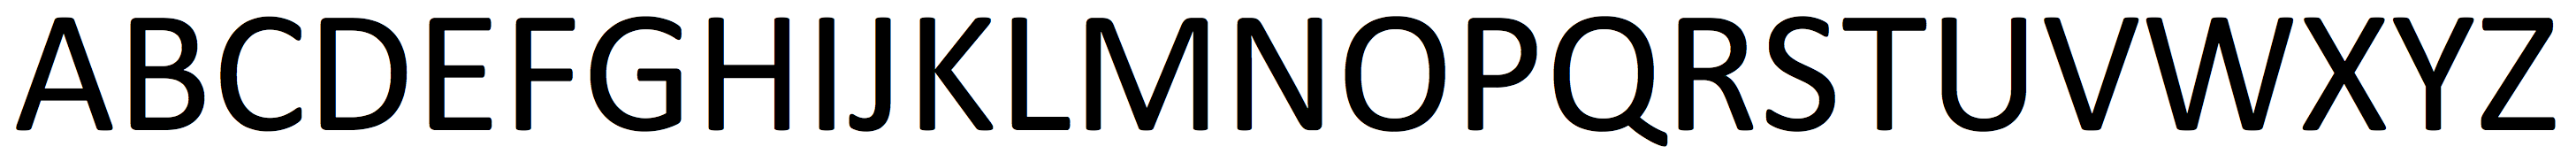
\includegraphics{alphabet.png}
\end{image}
\begin{freeResponse}
\begin{hint}
%\begin{tikzpicture}
%  \node {\scalebox{10}{\textsf{K}}};
%\end{tikzpicture}
\begin{itemize}
\item Vertical line symmetry:  A, H, I, M, O, T, U, V, W, X, Y
\item Horizontal line symmetry:  B, C, D, E H, I, K, O, X  
\item $180^\circ$ rotational symmetry: H, I, N, O, S, X, Z
\item None: F, G, J, L, P, Q, R.  
\end{itemize}
Notes:  (1) In many fonts that look much the same, the K has no symmetry.  (2) In this font, the O is slightly taller than it is wide.  If it were a circle, there would be more symmetry.  (See later problem.)
\end{hint}
\end{freeResponse}
\end{question}

\begin{question}
Write the words COKE and PEPSI in capital letters so that they read vertically.  Use a mirror to look at a reflection of the words.  What is different about the reflections of the two words?  Explain.  
\begin{freeResponse}
\begin{hint}
If the K has horizontal line symmetry in the font, then all the letters in COKE have horizontal line symmetry, which becomes vertical line symmetry when the word is written vertically. PEPSI, on the other hand, has several letters without that symmetry.  
\end{hint}
\end{freeResponse}
\end{question}

\begin{question}
Indicate the number of symmetries of the following figures: 
\begin{enumerate}
\item An equilateral triangle $\answer{6}$
\item An isosceles triangle that is not equilateral $\answer{2}$
\item A square $\answer{8}$
\item A rectangle that is not a square $\answer{4}$
\item A rhombus that is not a square $\answer{4}$
\item A (non-special) parallelogram $\answer{2}$
\item A regular $n-$gon $\answer{2n}$
\end{enumerate}
\end{question}

\begin{question}
Describe all of the symmetries of the following figures: 
\begin{enumerate}
\item An equilateral triangle
\item An isosceles triangle that is not equilateral
\item A square
\item A rectangle that is not a square
\item A rhombus that is not a square
\item A (non-special) parallelogram
\item A regular $n$-gon
\end{enumerate}
\begin{freeResponse}
\begin{hint}
\end{hint}
\end{freeResponse}
\end{question}


\begin{question}
We often say a figure is ``symmetric'' when we notice that it has symmetry, but now we want to be more precise:  

A \textbf{symmetry} of a figure is a \wordChoice{\choice{reflection}\choice{rotation}\choice[correct]{transformation}\choice{translation}} 
that maps a figure 
\wordChoice{\choice{to its opposite}\choice[correct]{onto itself}\choice{to another figure}}.  
\end{question}

\begin{question}
Explain why a sequence of two symmetries of a figure must also be a symmetry of that figure.  
\begin{freeResponse}
\begin{hint}
If a transformation T1 maps a figure onto itself and another transformation T2 maps the figure onto itself, then T1 followed by T2 also maps the figure onto itself.  

The first transformation leaves the figure unchanged and the second transformation leaves the figure unchanged, so the sequence of two transformations leaves the figure unchanged.  
\end{hint}
\end{freeResponse}
\end{question}

\begin{question}
Explain why the identity transformation should be considered a symmetry of \emph{any} figure.   
\begin{freeResponse}
\begin{hint}
The identity transformation satisfies the definition of a symmetry: It maps the figure onto itself. 

If a figure has reflection symmetry $R_k$ about a line $k$, then $R_k$ followed by $R_k$ is the identity transformation.  And by the previous result, this sequence of symmetries must also be a symmetry.  

If a figure has rotational symmetry $R_\alpha$ by some angle $\alpha$ about some center, then it must also have 

Note: If the identity transformation is the \emph{only} transformation of a figure, we usually say the figure is asymmetric or has no symmetry.  
\end{hint}
\end{freeResponse}
\end{question}


Symmetries of polygons.  

\begin{question}
Suppose that quadrilateral $ABCD$ has exactly one rotation symmetry (other than the identity transformation) and no reflection symmetry.  What kind(s) of quadrilateral could it be?  Explain your reasoning.  
\end{question}

\begin{question}
Suppose that quadrilateral $ABCD$ has exactly one reflection symmetry and no rotation symmetry (other than the identity transformation).  What kind(s) of quadrilateral could it be?  Explain your reasoning.  
\end{question}

\begin{question}
What are the symmetries of a circle? 
\begin{freeResponse}
\begin{hint}
A circle has rotational symmetry by any angle about its center.  A circle has reflection symmetry about any line through its center.  A circle does not have translation symmetry.  
\end{hint}
\end{freeResponse}
\end{question}

\begin{question}
How can you use the symmetries of a circle to determine whether a figure is indeed a circle?  
\begin{freeResponse}
\begin{hint}
Perform any of the symmetry transformations to be sure that the circle is actually mapped onto itself.  
\end{hint}
\end{freeResponse}
\end{question}

\begin{question}
What are the symmetries of a line?  
\begin{enumerate}
\item Describe all translation symmetries.  
\item Describe all rotation symmetries.
\item Describe two types of reflection symmetries.
\item Given a line, describe a rotation symmetry and a reflection symmetry that have the same effect on a line.  How do the corresponding transformations differ in what they do to the surrounding space?  
\end{enumerate}
\begin{freeResponse}
\begin{hint}
A line has translation symmetry by a vector of any length parallel to the line.  A line has $180^\circ$ rotational symmetry about any point on the line.  A line has reflection symmetry about any perpendicular to the line.  
\end{hint}
\end{freeResponse}
\end{question}

\begin{question}
How can you use the symmetries of a line to determine whether a figure is indeed a line? 
\begin{freeResponse}
\begin{hint}
Perform any of the symmetry transformations to be sure that the line is actually mapped onto itself.  
\end{hint}
\end{freeResponse}
\end{question}

\begin{question}
Find some tessellations.  For each tessellation, describe all of its symmetries.  
\begin{freeResponse}
\begin{hint}
\end{hint}
\end{freeResponse}
\end{question}



\end{document}
